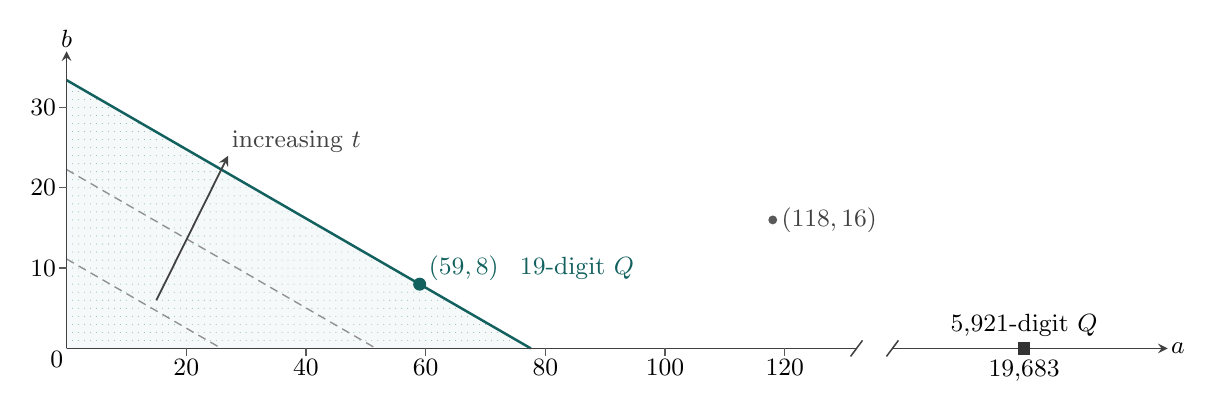
\begin{tikzpicture}[
    x=.76mm, y=1.02mm, font=\small,
    axis/.style={draw=black!75, line width=.55pt},
    tick/.style={draw=black!65, line width=.45pt},
    every node/.style={inner sep=1pt},
    >=stealth
]
\definecolor{productTeal}{HTML}{12615F}
\pgfmathsetmacro{\costRatio}{ln(5)/ln(2)}
\pgfmathsetmacro{\aIntercept}{59+8*\costRatio}
\pgfmathsetmacro{\bIntercept}{59/\costRatio+8}

% The row b contains the integers 0 <= a <= 59 + (8-b) log_2(5).
\fill[productTeal!4] (0,0) -- (\aIntercept,0) -- (0,\bIntercept) -- cycle;
\foreach \b in {0,...,33}{
    \pgfmathtruncatemacro{\lastA}{floor(59+(8-\b)*\costRatio)}
    \path[fill=productTeal!46] \foreach \a in {0,...,\lastA}
        {(\a,\b) circle[radius=.19pt]};
}
\foreach \portion in {1/3,2/3}{
    \draw[black!43, densely dashed, line width=.5pt]
        (0,{\portion*\bIntercept}) -- ({\portion*\aIntercept},0);
}
\draw[productTeal, line width=.9pt] (0,\bIntercept) -- (\aIntercept,0);
\draw[->, black!74, line width=.65pt] (15,6) -- (27,24)
    node[above right] {increasing $t$};

% The axis is linear through a = 130. Only the isolated axis minimum
% is shown to the right of the break.
\draw[axis,->] (0,0) -- (0,37) node[above] {$b$};
\draw[axis] (0,0) -- (132,0);
\draw[axis,->] (138,0) -- (184,0) node[right] {$a$};
\draw[axis] (131,-1) -- (133,1) (137,-1) -- (139,1);
\node[below left] at (0,0) {$0$};
\foreach \a in {20,40,60,80,100,120}
    \draw[tick] (\a,0) -- ++(0,-.9) node[below] {$\a$};
\foreach \b in {10,20,30}
    \draw[tick] (0,\b) -- ++(-1.2,0) node[left] {$\b$};

\fill[productTeal] (59,8) circle[radius=2.35pt];
\node[above right, text=productTeal] at (60,8)
    {$(59,8)$ \enspace 19-digit $Q$};
\fill[black!65] (118,16) circle[radius=1.6pt];
\node[right=2pt, text=black!75] at (118,16) {$(118,16)$};

\node[rectangle, fill=black!80, inner sep=0pt, minimum size=4.4pt] at (160,0) {};
\node[above=3pt] at (160,0) {5,921-digit $Q$};
\node[below=3pt] at (160,0) {$19{,}683$};
\end{tikzpicture}
